\documentclass[10pt]{article}
\usepackage[a4paper,margin=1.4cm,top=1.2cm,bottom=1.2cm]{geometry}
\usepackage{amsmath,amssymb,mathtools}
\usepackage{tikz}
\usepackage[dutch]{babel}
\usepackage[T1]{fontenc}
\usepackage{lmodern}
\usepackage{xcolor}
\usepackage[most]{tcolorbox}
\usepackage{enumitem}
\usepackage{booktabs}
\usepackage{multicol}
\usepackage{fancyhdr}
\usetikzlibrary{calc,patterns,decorations.pathmorphing,arrows.meta}

% ---------- Colors ----------
\definecolor{navy}{HTML}{13284A}
\definecolor{accent}{HTML}{2E75B6}
\definecolor{keyfill}{HTML}{EAF1FB}
\definecolor{keyline}{HTML}{2E75B6}
\definecolor{tipfill}{HTML}{FBF3E2}
\definecolor{tipline}{HTML}{D9A441}
\definecolor{warnfill}{HTML}{FBEAEA}
\definecolor{warnline}{HTML}{C0504D}
\definecolor{steel}{HTML}{9BA7B4}
\definecolor{ink}{HTML}{222831}

\color{ink}

% ---------- Header / footer ----------
\pagestyle{fancy}
\fancyhf{}
\renewcommand{\headrulewidth}{0pt}
\fancyfoot[L]{\footnotesize\color{steel}Formularium Sterkteleer}
\fancyfoot[R]{\footnotesize\color{steel}p.\ \thepage}
\setlength{\parindent}{0pt}
\setlength{\parskip}{1pt}

% ---------- Section style ----------
\newcommand{\sectionbar}[2]{%
\vspace{3pt}%
\begin{tcolorbox}[colback=navy,colframe=navy,boxrule=0pt,arc=2pt,left=6pt,right=6pt,top=3pt,bottom=3pt]
\color{white}\large\bfseries #1\hfill{\normalsize\mdseries\color{white!75!navy}#2}
\end{tcolorbox}%
\vspace{1pt}}

\newcommand{\subhead}[1]{\vspace{2pt}{\color{navy}\bfseries #1}\par\vspace{1pt}}

% key formula box (parate kennis)
\newtcolorbox{key}[1][]{colback=keyfill,colframe=keyline,boxrule=0.8pt,arc=2pt,
  left=6pt,right=6pt,top=3pt,bottom=3pt,#1}
\newtcolorbox{tipbox}{colback=tipfill,colframe=tipline,boxrule=0.6pt,arc=2pt,
  left=6pt,right=6pt,top=3pt,bottom=3pt}
\newtcolorbox{warnbox}{colback=warnfill,colframe=warnline,boxrule=0.6pt,arc=2pt,
  left=6pt,right=6pt,top=3pt,bottom=3pt}

\newcommand{\dd}{\,\mathrm{d}}

\begin{document}

% ===================== TITLE =====================
\begin{tcolorbox}[colback=navy,colframe=navy,boxrule=0pt,arc=3pt,left=12pt,right=12pt,top=8pt,bottom=8pt]
\color{white}
{\Huge\bfseries Formularium Sterkteleer}\\[2pt]
{\large FEO $\cdot$ Navier $\cdot$ Elastische energie $\cdot$ Stabiliteit $\cdot$ Torsie}\\[1pt]
{\footnotesize\color{white!80!navy} Samenvatting op basis van eigen notities + cursus (prof.\ R.\ Boonen). Ingekaderde formules = parate kennis.}
\end{tcolorbox}
\vspace{2pt}

% ===================================================================
\sectionbar{1. Buiging van balken --- Methode van Navier}{rechte balken, symmetrische doorsnede (I moet niet percee constant zijn)}

Doel: \textbf{hoekvervorming $\alpha(x)$ and doorbuiging $y(x)$} (klein verondersteld) bepalen voor \textbf{rechte balken} bij willekeurige belasting. Vertrek altijd van de \textbf{momentenvergelijking}. Werkt voor statische én hyperstatische constructies.

\begin{multicols}{2}
\begin{key}
\textbf{Differentiaalvergelijkingen van Navier:}
\[ \frac{\dd\alpha}{\dd x}=\frac{M}{EI}\qquad \frac{\dd^{2}y}{\dd x^{2}}=\frac{M}{EI}\]
In integrale vorm (vergeet de constanten niet!):
\[ \alpha(x)=\int\frac{M}{EI}\dd x+\alpha_0\]
\[ y(x)=\int \alpha(x)\dd x+y_0\]
\end{key}

\columnbreak

\subhead{Stappenplan}
\begin{enumerate}[leftmargin=1.4em,itemsep=0pt,topsep=1pt]
\item \textbf{VLS} $\rightarrow$ tekenconventie, reactiekrachten en -momenten op de balk.
\item \textbf{Statica} $\rightarrow$ evenwichtsvergelijkingen $\sum F\!=\!0,\ \sum M\!=\!0$.
\item \textbf{Momentenvergelijking} $M(x)$ via ``wandeling over de balk''.
\item Tweemaal integreren $\rightarrow \alpha(x),\ y(x)$.
\item \textbf{Randvoorwaarden} invullen $\rightarrow$ integratieconstanten.
\end{enumerate}
\end{multicols}

\vspace{-4pt}
\begin{multicols}{2}

\subhead{Randvoorwaarden per steunpunt}

\begin{center}
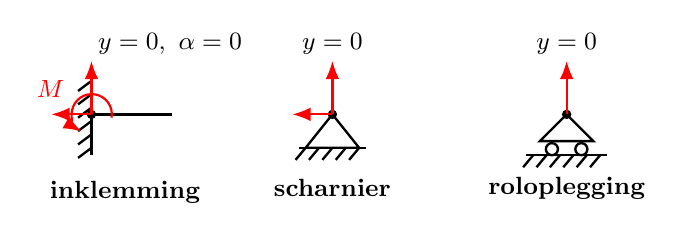
\begin{tikzpicture}[
    scale=0.85,
    line width=0.85pt,
    >=Latex,
    every node/.style={font=\small}
]
%====================================================
% INKLEMMING
%====================================================
\begin{scope}[shift={(0,0)}]
\draw (0,-0.6) -- (0,0.6);
\foreach \y in {-0.5,-0.3,-0.1,0.1,0.3,0.5}
{
    \draw (0,\y) -- (-0.2,\y-0.15);
}
\draw (0,0) -- (1.2,0);
\fill (0,0) circle (2pt);
\draw[red,->,thick] (0,0) -- (0,0.8);
\draw[red,->,thick] (0,0) -- (-0.6,0);
\draw[red,->,thick] (0.3,-0.05) arc (-10:240:0.3);
\node[red, anchor=south east] at (-0.25,0.1) {$M$};
\node[anchor=south west, inner sep=2pt] at (0,0.8) {$y=0,\ \alpha=0$};
\node[font=\small\bfseries, anchor=north] at (0.5,-0.85) {inklemming};
\end{scope}

%====================================================
% SCHARNIER
%====================================================
\begin{scope}[shift={(3.6,0)}]
\draw (0,0) -- (-0.4,-0.5) -- (0.4,-0.5) -- cycle;
\draw (-0.5,-0.5) -- (0.5,-0.5);
\foreach \x in {-0.4,-0.2,0,0.2,0.4}
{
    \draw (\x,-0.5) -- (\x-0.15,-0.68);
}
\fill (0,0) circle (2pt);
\draw[red,->,thick] (0,0) -- (0,0.8);
\draw[red,->,thick] (0,0) -- (-0.6,0);
\node[anchor=south, inner sep=2pt] at (0,0.8) {$y=0$};
\node[font=\small\bfseries] at (0,-1.1) {scharnier};
\end{scope}

%====================================================
% ROLOPLEGGING
%====================================================
\begin{scope}[shift={(7.1,0)}]
\draw (0,0) -- (-0.4,-0.4) -- (0.4,-0.4) -- cycle;
\draw (-0.22,-0.52) circle (0.09);
\draw (0.22,-0.52) circle (0.09);
\draw (-0.6,-0.61) -- (0.6,-0.61);
\foreach \x in {-0.5,-0.3,-0.1,0.1,0.3,0.5}
{
    \draw (\x,-0.61) -- (\x-0.15,-0.79);
}
\fill (0,0) circle (2pt);
\draw[red,->,thick] (0,0) -- (0,0.8);
\node[anchor=south, inner sep=2pt] at (0,0.8) {$y=0$};
\node[font=\small\bfseries] at (0,-1.1) {roloplegging};
\end{scope}
\end{tikzpicture}
\end{center}

\columnbreak

\subhead{Verschijnfunctie $\delta(x-a)$ (singulariteit)}
Activeert een term zodra $x>a$:
\[ \delta(x-a)=\begin{cases}1 & x>a\\[1pt]0 & x<a\end{cases}\quad(\text{ook genoteerd } \langle x-a\rangle)\]
Gedraagt zich bij integreren/afleiden als een \textbf{constante}:
\[ \tfrac{\dd}{\dd x}\!\big[f(x)\delta(x{-}a)\big]=\tfrac{\dd f}{\dd x}\,\delta(x{-}a)\]
\[ \int f(x)\,\delta(x{-}a)\dd x=\delta(x{-}a)\!\int f(x)\dd x\]
\end{multicols}

\begin{warnbox}
\textbf{Let op bij een extern moment $M$:} in $M(x)$ staat $M\,\delta(x-a)$, maar om correct te integreren schrijf je dit als $M\,(x-a)^{0}\,\delta(x-a)$. \emph{Niet} $M\,x\,\delta(x-a)$ --- anders zou de positie van $M$ geen effect hebben op de vervorming.
\end{warnbox}

% ===================================================================
\sectionbar{2. Elastische energie (Niet Plastisch!) \& stelling van Castigliano}{energie bekend $\rightarrow$ belasting/vervorming}

\begin{multicols}{2}
\textbf{Wanneer gebruiken?} Wanneer noch belasting noch vervorming op voorhand gekend is, enkel de \textbf{energie} (schok, val, stoot, optakelen van een last). Ook voor stabiliteit (knik) en speciale constructies (gekromde balken).

\begin{center}\footnotesize
\begin{tabular}{@{}lll@{}}
\toprule
Bekend & Gezocht & Methode\\\midrule
Belasting & Vervorming & Navier\\
Vervorming & Belasting & Navier\\
Energie & Belasting \& vervorming & \textbf{Energie}\\
\bottomrule
\end{tabular}
\end{center}

\columnbreak

\begin{key}
\textbf{Potentiële energie = arbeid:}
\[ E_p=W=\int_S B\dd q\ = \int_{A}^{B} F\dd s\]
$B$ = kracht óf moment, $q$ = verplaatsing óf hoekverdraaiing. Dit is een \textbf{bepaalde} integraal (een getal).
\[ \dd W=\frac{\sigma^{2}}{2E}\dd V \qquad \dd W=\frac{\tau^{2}}{2G}\dd V\]
\end{key}
\end{multicols}
\newpage
\subhead{Elastische energie voor de 4 basisbelastingen}
\begin{multicols}{4}
\begin{key}[left=4pt,right=4pt,top=3pt,bottom=3pt]
\centering \textbf{Trek}\\[2pt]
$\displaystyle W=\frac{F^{2}l}{2EA}$
\end{key}
\begin{key}[left=4pt,right=4pt,top=3pt,bottom=3pt]
\centering \textbf{Afschuiving}\\[2pt]
$\displaystyle W=\frac{F^{2}h}{2GA}$
\end{key}
\begin{key}[left=4pt,right=4pt,top=3pt,bottom=3pt]
\centering \textbf{Torsie}\\[2pt]
$\displaystyle W=\frac{M_w^{2}\,l}{2GI_p}$
\end{key}
\begin{key}[left=4pt,right=4pt,top=3pt,bottom=3pt]
\centering \textbf{Buiging}\\[2pt]
$\displaystyle W=\!\int_l\!\frac{M(x)^{2}}{2EI}\dd x$
\end{key}
\end{multicols}

\begin{multicols}{2}
\begin{key}
\textbf{Stelling van Castigliano:}
\[ y=\frac{\partial W}{\partial F}\qquad \alpha=\frac{\partial W}{\partial M}\]
Geeft de verplaatsing op de plaats én in de richting van $F$ (resp.\ hoek bij $M$).
\end{key}

\columnbreak

\subhead{Dummy-belasting}
Geen kracht op de gezochte plaats? Breng een \textbf{dummy} $D$ (of dummy-moment) aan:
\[ y_D=\frac{1}{EI}\int_l M\,\frac{\partial M}{\partial D}\dd x\]
$D$ staat enkel in $M(x)$ om te kunnen afleiden naar $D$; \textbf{stel $D=0$} direct na het afleiden, vóór het integreren.
\end{multicols}

\begin{tipbox}
\textbf{Bij het integreren werk je met BEPAALDE integralen} $\to$ splits het domein op per verschijnfunctie: $\delta(x-a)$ start de integratie pas vanaf $x=a$. Vergeet de dubbele producten niet bij het kwadrateren van $M(x)$! Product van verschijnfuncties: $\delta(x{-}a)\,\delta(x{-}b)=\delta(x{-}b)$ als $b>a$.
\end{tipbox}

\subhead{Gekromde balken (Navier niet geldig $\to$ Castigliano)}
Curve $S$ in één plaatsvariabele (hoek $\theta$ of $s$), moment $M(\theta)$, met $\dd s=R\dd\theta$ voor een cirkelboog:
\[
\begin{aligned}
W = \int_S\frac{M(s)^2}{2EI}\dd s \quad && 
x = \int_S\frac{M(s)}{EI}\frac{\partial M_s}{\partial F_x}\dd s \quad && 
y = \int_S\frac{M(s)}{EI}\frac{\partial M_s}{\partial F_y}\dd s \quad && 
\varphi = \int_S\frac{M(s)}{EI}\frac{\partial M_s}{\partial M_0}\dd s
\end{aligned}
\]

% ===================================================================
\sectionbar{3. Stabiliteit van constructies \& knik}{Lyapunov $\cdot$ Euler}

\begin{multicols}{2}
\subhead{Evenwicht via Lyapunov}
Drie soorten evenwicht: \emph{stabiel} (keert terug), \emph{onverschillig} (blijft), \emph{onstabiel} (loopt weg).
\begin{key}
\[ V=E_p-W\]
\textbf{Evenwicht:}\ $\dfrac{\partial V}{\partial q}=0$ \quad ($q$ = plaatscoördinaat)\\[2pt]
\textbf{Stabiliteit:}\ $S=\dfrac{\partial^{2}V}{\partial q^{2}}$
\[ S>0\ \text{stabiel}\quad S<0\ \text{onstabiel}\quad S=0\ \text{onverschillig}\]
\end{key}
Elk evenwichtspunt afzonderlijk in $S$ invullen en het teken beoordelen.

\columnbreak

\subhead{Knik van balken (Euler)}
Buigingsenergie $E_p=\int_l \frac{M^2}{2EI}\dd l$ met $\frac{\dd^2y}{\dd x^2}=\frac{M}{EI}$ levert de DV $y''''-\frac{F}{EI}y''=0$. De knikvorm is een (halve) sinus.
\begin{key}
\textbf{Knikformule van Euler:}
\[ F_k=\frac{\pi^{2}EI}{(c\,l)^{2}}\]
$c\,l$ = vrije kniklengte (afh.\ van de oplegging).
\end{key}
\begin{warnbox}
$I$ is het \textbf{KLEINSTE} traagheidsmoment ($I_x\neq I_y$): de balk knikt om de zwakste as. Controleer dat $\sigma=F_k/A$ onder de elasticiteitsgrens blijft, anders geldt Euler niet (plastische knik).
\end{warnbox}
\end{multicols}

\subhead{Vier standaardgevallen (waarde van $c$)}
\begin{center}
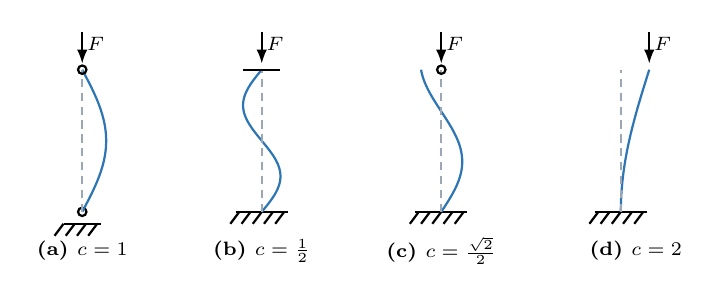
\begin{tikzpicture}[line width=0.8pt,scale=0.95]
\def\H{1.9}
\newcommand{\ground}[1]{\draw (#1-0.35,0)--(#1+0.35,0); \foreach \i in {-0.3,-0.15,0,0.15,0.3} \draw (#1+\i,0)--(#1+\i-0.12,-0.16);}
\newcommand{\pin}[1]{\draw (#1,0.0) circle (1.6pt); \draw(#1-0.25,-0.16)--(#1+0.25,-0.16); \foreach \i in {-0.2,-0.05,0.1,0.25} \draw(#1+\i-0.05,-0.16)--(#1+\i-0.17,-0.32);}
\begin{scope}[shift={(0,0)}]
  \pin{0}
  \draw[accent] plot[domain=0:\H,samples=40] ({0.32*sin(180*\x/\H)},\x);
  \draw[densely dashed,steel] (0,0)--(0,\H);
  \draw (0,\H) circle (1.6pt);
  \draw[-{Latex[length=1.8mm]}] (0,\H+0.5)--(0,\H+0.08); \node[font=\scriptsize] at (0.18,\H+0.35){$F$};
  \node[font=\scriptsize\bfseries] at (0,-0.52){(a) $c=1$};
\end{scope}
\begin{scope}[shift={(2.4,0)}]
  \ground{0}
  \draw[accent] plot[domain=0:\H,samples=60] ({0.25*sin(360*\x/\H)},{\x});
  \draw[densely dashed,steel] (0,0)--(0,\H);
  \draw (-0.25,\H)--(0.25,\H);
  \draw[-{Latex[length=1.8mm]}] (0,\H+0.5)--(0,\H+0.08); \node[font=\scriptsize] at (0.18,\H+0.35){$F$};
  \node[font=\scriptsize\bfseries] at (0,-0.52){(b) $c=\tfrac12$};
\end{scope}
\begin{scope}[shift={(4.8,0)}]
  \ground{0}
  \draw[accent] plot[domain=0:\H,samples=60] ({0.28*sin(255*\x/\H)},\x);
  \draw[densely dashed,steel] (0,0)--(0,\H);
  \draw (0,\H) circle (1.6pt);
  \draw[-{Latex[length=1.8mm]}] (0,\H+0.5)--(0,\H+0.08); \node[font=\scriptsize] at (0.18,\H+0.35){$F$};
  \node[font=\scriptsize\bfseries] at (0,-0.52){(c) $c=\tfrac{\sqrt2}{2}$};
\end{scope}
\begin{scope}[shift={(7.2,0)}]
  \ground{0}
  \draw[accent] plot[domain=0:\H,samples=40] ({0.38*(1-cos(90*\x/\H))},\x);
  \draw[densely dashed,steel] (0,0)--(0,\H);
  \draw[-{Latex[length=1.8mm]}] (0.38,\H+0.5)--(0.38,\H+0.08); \node[font=\scriptsize] at (0.56,\H+0.35){$F$};
  \node[font=\scriptsize\bfseries] at (0.2,-0.52){(d) $c=2$};
\end{scope}
\end{tikzpicture}
\end{center}
\vspace{-6pt}
\begin{center}\footnotesize
(a) beide scharnierend \quad (b) beide ingeklemd \quad (c) ingeklemd--scharnierend \quad (d) ingeklemd--vrij
\end{center}
\newpage
\subhead{Oppervlaktetraagheidsmoment van een samengestelde doorsnede (Steiner)}
\begin{multicols}{2}
\begin{key}
\[ I_x=\sum_i\!\Big(I_{c,i}+A_i\,(y_i-\bar y)^2\Big)\]
\[ I_y=\sum_i\!\Big(I_{c,i}+A_i\,(x_i-\bar x)^2\Big)\]
met de zwaartepunten
\[ \bar y=\frac{\sum A_i y_i}{\sum A_i}\qquad \bar x=\frac{\sum A_i x_i}{\sum A_i}\]
\end{key}

\columnbreak

\textbf{Regel:} cube altijd de maat \emph{loodrecht} op de as.\\
Rechthoek (breedte $b$, hoogte $h$):
\[ I_{x,c}=\frac{b\,h^{3}}{12}\qquad I_{y,c}=\frac{h\,b^{3}}{12}\]
$d_i$ = afstand van de deel-centroïde tot de \textbf{totale} centroïdale as. Bereken dus \textbf{eerst} $\bar x,\bar y$. Bij symmetrie valt de as vanzelf op het midden $\to$ geen berekening nodig in die richting. Gaten tel je negatief mee.
\end{multicols}

% ===================================================================
\sectionbar{4. Torsie van niet-ronde profielen}{wringmoment $\rightarrow$ schuifspanning}

Torsie ontstaat door een wringmoment $M_w$, overgebracht via schuifspanningen. Bij niet-ronde profielen \emph{welft} de doorsnede (ongeacht de lengte). De wringhoek $\varphi$ geldt voor alle onderstaande profielen.

\vspace{2pt}
\begin{multicols}{3}
\begin{key}[height=98pt]
\centering \textbf{Rond profiel \& Hoek}\\[6pt]
$\displaystyle \tau = \frac{M_w\,r}{I_p}$ \text{(alleen bij rond!)} \\[12pt]
$\displaystyle \varphi = \frac{M_w\,l}{G\,I_p} \text{(geld altijd!)}$
\end{key}

\begin{key}[height=98pt]
\centering \textbf{Gesloten koker (Bredt)}\\[4pt]
$\displaystyle \tau_{\max} = \frac{M_w}{2A_0\,t_{\min}}$ \\[8pt]
$\displaystyle I_p = \frac{4A_0^{2}}{\displaystyle\oint_S \frac{\dd s}{t(s)}}$
\end{key}

\begin{key}[height=98pt]
\centering \textbf{Open profiel}\\[6pt]
$\displaystyle \tau_{\max} = \frac{M_w\,t_{\max}}{I_p}$ \\[16pt]
$\displaystyle I_p = \frac{1}{3}\int_S t(s)^{3}\dd s$
\end{key}
\end{multicols}

\subhead{Geometrische eigenschappen per type profiel}
\begin{tcolorbox}[colback=white, colframe=steel!30, boxrule=0.5pt, arc=2pt, left=6pt, right=6pt, top=4pt, bottom=4pt]
\footnotesize
\textbf{Gesloten kokerprofiel:} $A_0$ = ingesloten oppervlak begrensd door de \textbf{middellijn}.\\
\textbf{Open profiel:} Een wand verliest aan elke \emph{verbonden} kant $\tfrac{\text{aangrenzende dikte}}{2}$. Gesloten: beide kanten verbonden ($B-d$). Open: één vrij uiteinde ($B-\tfrac{d}{2}$).
\end{tcolorbox}

\subhead{Uitgewerkte voorbeelden}
\begin{multicols}{2}

% Closed O-profile
\begin{minipage}[t]{\linewidth}
\textbf{Gesloten O-profiel}\ ($B{=}60$, $H{=}100$, flens $D{=}8$, wand $d{=}6$ mm):
\begin{center}
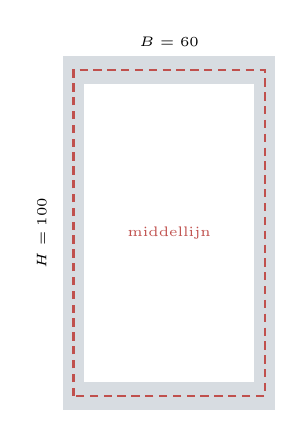
\begin{tikzpicture}[scale=0.045,line width=0.6pt]
\fill[steel!40] (0,0) rectangle (60,100);
\fill[white] (6,8) rectangle (54,92);
\draw[warnline,densely dashed,line width=0.8pt] (3,4) rectangle (57,96);
\node[font=\tiny] at (30,104){$B=60$};
\node[font=\tiny,rotate=90] at (-6,50){$H=100$};
\node[font=\tiny] at (30,50){\textcolor{warnline}{middellijn}};
\end{tikzpicture}
\end{center}
\vspace{-4pt}
{\footnotesize
\[ A_0=(B{-}d)(H{-}D)=54\cdot92=4968\ \text{mm}^2\]
\[ \oint\!\frac{\dd s}{t}=2\frac{B{-}d}{D}+2\frac{H{-}D}{d}=2\tfrac{54}{8}+2\tfrac{92}{6}=44{,}17\]
\[ I_p=\frac{4A_0^2}{44{,}17}=2{,}235\cdot10^{-6}\ \text{m}^4\]}
\end{minipage}

\columnbreak

% Open C-profile
\begin{minipage}[t]{\linewidth}
\textbf{Open C-profiel}\ ($B{=}80$, $H{=}120$, flens $D{=}10$, wand $d{=}6$ mm):
\begin{center}
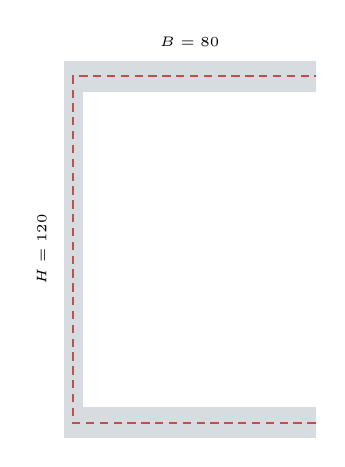
\begin{tikzpicture}[scale=0.04,line width=0.6pt]
\fill[steel!40] (0,0) rectangle (80,10);
\fill[steel!40] (0,0) rectangle (6,120);
\fill[steel!40] (0,110) rectangle (80,120);
\draw[warnline,densely dashed,line width=0.8pt] (80,5)--(3,5)--(3,115)--(80,115);
\node[font=\tiny] at (40,126){$B=80$};
\node[font=\tiny,rotate=90] at (-7,60){$H=120$};
\end{tikzpicture}
\end{center}
\vspace{-4pt}
{\footnotesize
\[ I_p=\tfrac{1}{3}\big(2(B{-}\tfrac{d}{2})D^{3}+(H{-}D)d^{3}\big)\]
\[ = \tfrac{1}{3}\big(2\cdot77\cdot10^{3}+110\cdot6^{3}\big)\]
\[ = \tfrac{1}{3}\cdot177\,760=59\,253\ \text{mm}^4\]}
\end{minipage}
\end{multicols}

\begin{tipbox}
\textbf{Gevaar van een las (vb.\ buis $D{=}80$, $d{=}6$):} barst de las, dan wordt een gesloten profiel plots open. $I_p$ daalt van $1{,}909\cdot10^{-6}$ naar $16\,738\cdot10^{-12}\,\text{m}^4 \Rightarrow \tau_{\max}$ wordt \textbf{18$\times$ hoger} en $\varphi$ \textbf{$\sim$100$\times$ groter}. Daarom: voor koppeloverdracht altijd naadloze (niet-gelaste) buis.
\end{tipbox}
\end{document}
